\documentclass[a4paper,12pt]{article}
%%%%%%%%%%%%%%%%%%%%%%%%%%%%%%%%%%%%%%%%%%%%%%%%%%%%%%%%%%%%%%%%%%%%%%%%%%%%%%%%%%%%%%%%%%%%%%%%%%%%%%%%%%%%%%%%%%%%%%%%%%%%%%%%%%%%%%%%%%%%%%%%%%%%%%%%%%%%%%%%%%%%%%%%%%%%%%%%%%%%%%%%%%%%%%%%%%%%%%%%%%%%%%%%%%%%%%%%%%%%%%%%%%%%%%%%%%%%%%%%%%%%%%%%%%%%
\usepackage{eurosym}
\usepackage{vmargin}
\usepackage{amsmath}
\usepackage{graphics}
\usepackage{epsfig}
\usepackage{subfigure}
\usepackage{fancyhdr}
\usepackage{listings}
\usepackage{framed}
\usepackage{graphicx}
\usepackage{amsmath}
\usepackage{chngpage}
%\usepackage{bigints}

%\setcounter{MaxMatrixCols}{10}

\begin{document}
	\large
	
\section*{Bokeh Tutorial — Styling and Appearance}

\subsection*{Preliminaraies}
\begin{framed}
\begin{verbatim}
from bokeh.io import output_notebook, show
from bokeh.plotting import figure

output_notebook()
# BokehJS successfully loaded.
\end{verbatim}
\end{framed}

%===================================================================== %

\subsection{Colours}
There are many places where you may need to specify colors. Bokeh can accept colors in a variety of different ways:
\begin{enumerate}
\item any of the 147 named CSS colours, e.g 'green', 'indigo'
\item an \textit{\textbf{RGB(A)}} hex value, e.g., '$\#FF0000$', '$\#44FF66$'
\item a 3-tuple of integers (r,g,b) between 0 and 255
\item a 4-tuple of (r,g,b,a) where r, g, b are integers between 0 and 255 and a is a floating point value between 0 and 1
\end{enumerate}

%============================================================= %
\subsection{Properties}
Regardless of what API (models, plotting, or charts) is used to create a Bokeh plot, styling the visual aspects of the plot can always be accomplished by setting attributes on the Bokeh model objects that comprise the resulting plot. Visual properties come in three kinds: line, fill, and text properties. 
% For full information with code and examples see the Styling Visual Properties section of the user guide.


\subsubsection{Line Properties}
Set the visual appearance of lines. The most common are \texttt{line\_color}, \texttt{line\_alpha}, \texttt{line\_width} and \texttt{line\_dash}.

\subsubsection{Fill Properties}
Set the visual appearance of filled areas: \texttt{fill\_color} and \texttt{fill\_alpha}.

\subsubsection{Text Properties}
Set the visual appearance of lines of text. The most common are \texttt{text\_font}, \texttt{text\_font\_size}, text\_color, and \texttt{text\_alpha}.

Sometimes a prefix is used with property names, e.g. to distinguish between different line properties on the same object, or to give a more meaningful name. 

For example, to set the line width of the plot outline, you would say \texttt{myplot.outline\_line\_width = 2}.
%================================================================================================= %
\subsection{Plots}
Many top-level attributes of plots (outline, border, etc.) can be configured. See the Plots section of the styling guide for full information.

Here is an example that tweaks the plot outline:

\begin{framed}
\begin{verbatim}
# create a new plot with a title
p = figure(plot_width=400, plot_height=400)
p.outline_line_width = 7
p.outline_line_alpha = 0.3
p.outline_line_color = "navy"

p.circle([1,2,3,4,5], [2,5,8,2,7], size=10)

show(p)
	
\end{verbatim}
\end{framed}

\begin{figure}[h!]
\centering
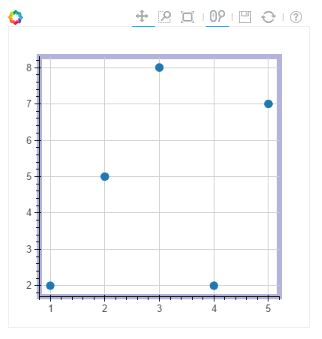
\includegraphics[width=0.7\linewidth]{images/04-plotoutline-01}
\end{figure}

\subsection*{EXERCISE}Create a plot of your own and customize several plot-level properties

% Axes


\subsection{Axes}

To style axes, you first must get ahold of Axis objects. The simplest way is to use some convenience methods on Plot: axis, xaxis, and yaxis. These methods return lists of axis objects:
\\
\begin{framed}
	\begin{verbatim}
>>> p.xaxis
[<bokeh.models.axes.LinearAxis at 0x106fa2390>]
\end{verbatim}
\end{framed}
However, you can set properties on all the elements of the list as if it was a single object:
\begin{framed}
	\begin{verbatim}
p.xaxis.axis_label = "Temperature"
p.axis.major_label_text_color = "orange"
\end{verbatim}
\end{framed}
These are referred to as "splattable" lists, and tab completion works on them as well.

Try out tab completion. Type p.xaxis.<press tab key> to see a list of attributes that can be set.
\begin{framed}
\begin{verbatim}
axis
line properties
axis_label
text properties
axis_label_standoff
major_label
text properties
orientation
major_tick
line_properties
major_tick_in
major_tick_out
minor_tick
line properties
minor_tick_in
minor_tick_out
\end{verbatim}
\end{framed}
As a simple first example, let's change the orientation of the major tick labels on both axes of a plot:
\begin{framed}
	\begin{verbatim}
from math import pi

p = figure(plot_width=400, plot_height=400)
p.x([1,2,3,4,5], [2,5,8,2,7], size=10, line_width=2)

p.xaxis.major_label_orientation = pi/4
p.yaxis.major_label_orientation = "vertical"

show(p)
\end{verbatim}
\end{framed}
The next example shows customizations on several of the different Axis properties at once:
\begin{framed}
	\begin{verbatim}
p = figure(plot_width=400, plot_height=400)
p.asterisk([1,2,3,4,5], [2,5,8,2,7], size=12, color="olive")

# change just some things about the x-axes
p.xaxis.axis_label = "Temp"
p.xaxis.axis_line_width = 3
p.xaxis.axis_line_color = "red"

# change just some things about the y-axes
p.yaxis.axis_label = "Pressure"
p.yaxis.major_label_text_color = "orange"
p.yaxis.major_label_orientation = "vertical"

# change things on all axes
p.axis.minor_tick_in = -3
p.axis.minor_tick_out = 6

show(p)
\end{verbatim}
\end{framed}	
%In [8]:
\subsection*{EXERCISE} 
Create a plot of your own and customize several axis properties
%There are further customizations possible. See the User Guide for more information on topics such as tick label formatting or limiting axis bounds.

%======================================================================================== %
\subsection{Grids}




\begin{framed}
\begin{verbatim}
# grid line properties
# band fill properties

p = figure(plot_width=400, plot_height=400)
p.circle([1,2,3,4,5], [2,5,8,2,7], size=10)

# change just some things about the x-grid
p.xgrid.grid_line_color = None

# change just some things about the y-grid
p.ygrid.grid_line_alpha = 0.5
p.ygrid.grid_line_dash = [6, 4]

show(p)
\end{verbatim}
\end{framed}
\begin{figure}[h!]
\centering
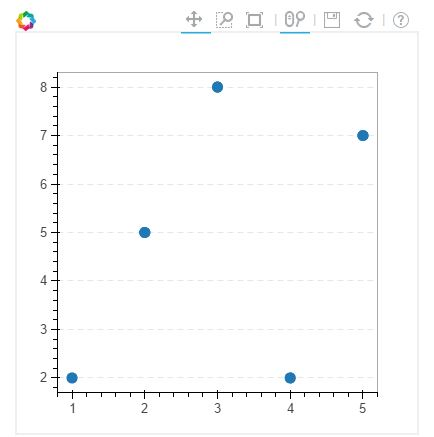
\includegraphics[width=0.7\linewidth]{images/04-grids-01}
\end{figure}

\begin{framed}
	\begin{verbatim}
In [10]:
p = figure(plot_width=400, plot_height=400)
p.circle([1,2,3,4,5], [2,5,8,2,7], size=10)

# change just some things about the x-grid
p.xgrid.grid_line_color = None

# change just some things about the y-grid
p.ygrid.band_fill_alpha = 0.1
p.ygrid.band_fill_color = "navy"

show(p)
\end{verbatim}
\end{framed}
\begin{figure}[h!]
	\centering
	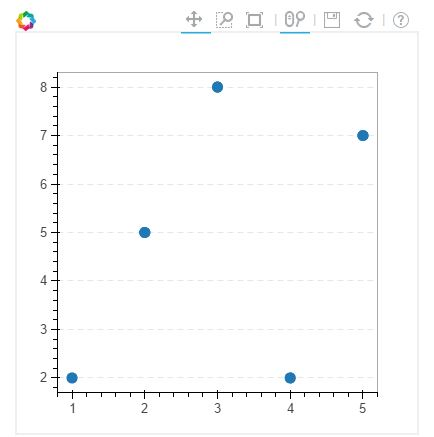
\includegraphics[width=0.7\linewidth]{images/04-grids-01}
\end{figure}
\subsection*{EXERCISE} Create a plot of your own and customize several grid properties.

%===================================================================================== %
\newpage
\subsection*{Legends}

\begin{framed}
\begin{verbatim}
In [12]:
import numpy as np

x = np.linspace(0, 4*np.pi, 100)
y = np.sin(x)

p = figure()

p.circle(x, y, legend="sin(x)")
p.line(x, y, legend="sin(x)")

p.line(x, 2*y, legend="2*sin(x)", line_dash=[4, 4], line_color="orange", line_width=2)

p.line(x, 3*y, legend="3*sin(x)", line_color="green")
p.square(x, 3*y, legend="3*sin(x)", fill_color="white", line_color="green")

p.legend.orientation = "bottom_left"

show(p)
\end{verbatim}
\end{framed}	
\begin{figure}[h!]
\centering
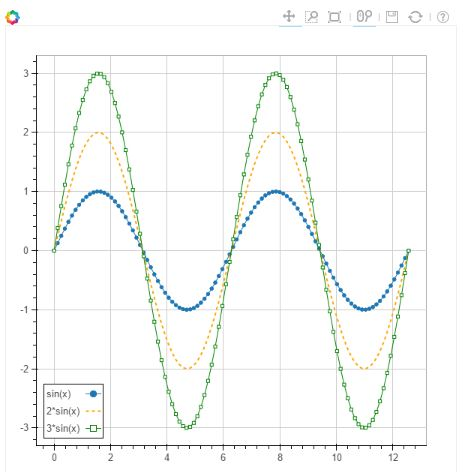
\includegraphics[width=0.7\linewidth]{images/04-legends-01}
\end{figure}

\subsection*{Exercise}
Create a plot of your own and add a legend

\end{document}
%Back to top
%This web site does not host notebooks, it only renders notebooks available on other websites.
%
%Delivered by Fastly, Rendered by Rackspace
%
%nbviewer GitHub repository.
%
%nbviewer version: 03d6df0
%
%IPython version: 4.0.0
%
%Rendered in a few seconds
